\chapter{Main Idea}
Hiding malware in data files can be done in a multitude of ways and for this thesis we choose to replicate an especially
interesting malware attack which occured in 2021. It was reported on by Hossein Jazi, senior threat intelligence
analyst with Malwarebytes in July 2021, on the company's blog. The article shared some important details about the malware 
itself, such as \acrfull{iocs} and addresses of the command and control servers, but also a thorough write-up of the mechanisms 
the malware used to drop a \acrfull{rat}.

The most notable part of the malware in our eyes was the fact it used an image conversion algorithm native to Microsoft
Windows in order to extract the payload in a relatively benign looking operation, so we decided to recreate it 
in the interest of scientific rigour and checking whether the exploit still works, or if changes have occurred
that make this kind of attack impossible.

The primary source for our research and recreation of the malware is the aforementioned article, which we have stuck to
as closely as possible throughout. However, this wasn't always possible, and we had to engineer a handful of tools
to make the malware work ourselves. 

We have left out a number of parts of the virus which we deemed irrelevant to our goals; we haven't recreated the lure
form or the original document form for example, as we don't find it necessary to create a convincing lure in order to
demonstrate the vulnerability being exploited.

As a final disclaimer, we replaced the malicious payload with a benign application, which does not harm the computer
that executes the malware. Since the focus of this work is hiding executable code within data files, we focus on
that mechanism, rather than the final malicious payload itself. The original malicious document extracted an encrypted
executable which decoded itself and loaded a second-stage payload into memory which established communication with a
command and control server.

\section{Malware Recreation}
The malware itself consisted of multiple separate mechanisms that come together to drop and execute a malicious payload
on the victim's machine. The following activity diagram shows the execution flow of the malware, 
with swimlanes for each individual part of the malware.

We classify this malware as a macro virus, so of course, the initial infection starts when the victim opens the macro
enabled document and allows the execution of macros. This is, naturally, something one should never do for security
reasons, and yet macro viruses remain a common infection vector for malware, with users often clicking the \emph{enable
macros} button out of habit, not realising the severity of their actions \cite{macro-viruses-users}.

\begin{figure}[H]
  \centering
  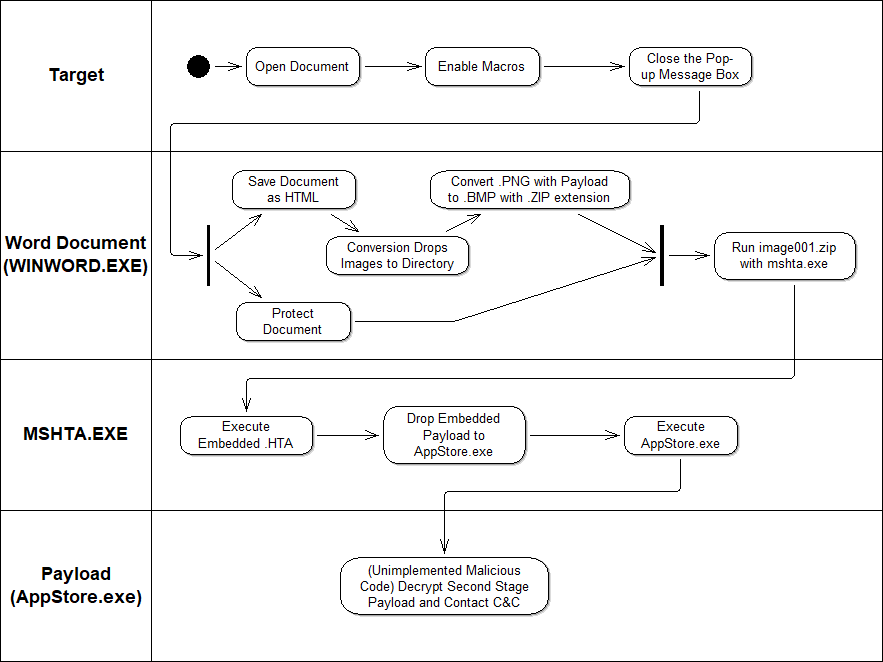
\includegraphics[width=0.9\textwidth]{figures/malware-process-graph.png}
  \label{process-graph}
  \caption{Malware process graph}
\end{figure}

After the victim enables macros, a message box pops up informing the user a demonstration of the payload dropping
mechanism will occur after they close the message box. In the original virus, this message box claimed that the user 
was using an older version of Microsoft Office \cite{jazi-article}. Coinciding with the roll-out of the new operating 
system Windows 11, we believe the purpose of this message box was for the victim to dismiss any performance loss their 
device may suffer during the payload extraction and attribute it to the document being made compatible with their version 
of Microsoft Office. 
We conclude this because when experimenting with differently sized payloads we observed a significant performance drop
on the device while the payload was extracted by \verb+mshta.exe+.

Regardless of what option the victim selects in the message box, the macro will continue execution. The macro obfuscates
key constants in order to avoid automated detection and to make analysis more difficult. The chosen obfuscation
methodology includes introducing encoded strings, misleading variable names as well as some excess declarations to 
serve as smoke and mirrors for analysts.

\begin{lstlisting}[language=VBScript, caption={Encoded strings in the macro}][H]
  MyCalc = "d2lubWdtdHM6Ly8uL3Jvb3QvY2ltdjI6V2luMzJfUHJvY2Vzcw==" ' winmgmts://./root/cimv2:Win32_Process
  Dim Calc As String : Calc = Decode(MyCalc)
  Dim MyValue As String : MyValue = "bXNodGE=" ' mshta
  Dim Value As String : Value = Decode(MyValue)
  Dim MyExt1 As String : MyExt1 = "emlw" ' zip
  Dim Ext1 As String : Ext1 = Decode(MyExt1)
\end{lstlisting}

The main purpose of the macro is to execute a payload loader and then remove all traces of its presence from the system.
It achieves this with a creative mechanism -- the document is saved as \acrshort{HTML}, which extracts the contents of the
document, most importantly for us the images, to a subdirectory, while appearing completely benign. The next misleading
step is a simple call to \verb+WIA_ConvertImage+, an image conversion function. This function is \emph{supposed} to
convert and image from one format to another, in this case \acrshort{PNG} to \acrshort{BMP}, but it in fact achieves a
more sinister goal. During the image conversion process, an embedded \verb+Zlib+ archive appended to the \acrshort{PNG}
image gets extracted, appending a \acrfull{HTA} document to the end of the resulting \acrshort{BMP} image.

In the final step of execution within Microsoft Word, the macro uses the \acrfull{mshta} executable to run the resulting
\acrshort{BMP} image and deleting all the artefacts left behind by the macro.

Handing off to \acrshort{mshta}, the malware runs a heavily obfuscated \acrshort{HTA} document which serves to drop the
payload. This is the most obfuscated part of the code we covered and while the unobfuscated code has less than 20 lines
of code, the obfuscated version has almost three times as many. The executable payload is also stored directly in the
\acrshort{HTA}, leading to a massively inflated line count if we count it, since even small executables serialise to
thousands of lines in the chosen serialisation method. 

This part of the malware uses a few quirks of the JavaScript language to make analysis even harder, chief among which is
the use of bracket notation in object access. Using the fact that all arrays in JavaScript are objects, their properties
can be accessed using bracket notation as well as dot notation, in short: \verb+foo.push()+ and \verb+foo['push']()+ are 
considered to be equivalent and equally valid notations. 
The malware further combines this by saving the property names in an array accessed via a special function that takes an 
input and converts it into a valid index. The array is also shuffled during execution for good measure. This all leads to 
severly worsened readability of function calls, such as \verb+e[_0x556975(0x1ec)]('MZ')+
\footnote{Unobfuscated: \texttt{file.Write('MZ')}.}, making analysis more difficult. % inline \verb doesn't work in footnote

The executable is stored in memory as an array of Unicode characters represented numerically, corresponding to the
\verb+unsigned short+ data type in C. This array is joined into a string using the JavaScript \verb+String.fromCharCode()+
function and then written to a file using a Microsoft JScript object, namely
\verb+ActiveXObject("Scripting.FileSystemObject")+, the same object used in the \acrshort{VBA} section of the malware.
Finally, the payload is executed using another Microsoft JScript object, \verb+ActiveXObject('WScript.Shell')+, which
hands off execution to the payload, \verb+AppStore.exe+.

\verb+AppStore.exe+ is where we stopped our implementation, as what happens next is essentially the virus' endgame. 
A malicious executable has been dropped onto the user's system and executed, the author is free to do as they please.
In the original attack, the payload loads a base 64 encrypted second stage payload into memory and decrypts it in order to
establish communications with a command and control server, with all the API requests between the infected device
and the command and control server being encrypted with a custom algorithm similar to one used in a previous incident
attributed to Lazarus \acrshort{APT} \cite{jazi-article}. 

% --------------------------------------------------
% Notes
% --------------------------------------------------
\begin{enumerate}
  \item Lazarus BMP RAT Analysis
  \item My re-implementation in key points
  \item Tests on different operating systems
    \begin{itemize}
      \item Current Windows systems
      \item EOL Windows systems
      \item Linux systems
      \item Running the malware \emph{outside} MS Office
    \end{itemize}
\end{enumerate}


